\subsection{Aimspice results} 
After running all the simulations we ended up with the power consumption shown in the figures \ref{fig:0.3_I1_I2}, \ref{fig:0.3_I3_I4} \ref{fig:0.6_I1_I2} and \ref{fig:0.6_I3_I4}. The dotes are the actual values simulated while the the lines are plotted using python function Polynomial.fit at 5 degrees to give us aid in visualise the trends regardig the variables.

\imagesidebyside{figures/aimspice/variableVDD/CSV/static_power_leakage_graph_I1.png}{Clk:0, Data:0, Reset:1, Q:1}{figures/aimspice/variableVDD/CSV/static_power_leakage_graph_I2.png}{Clk:0, Data:1, Reset:1, Q:0}{Static leakage power when  $N_W=0.1u$, $N_L=0.1u$, $P_W=0.3u$ and $P_L=0.1u$}{0.3_I1_I2}{0.49}

\imagesidebyside{figures/aimspice/variableVDD/CSV/static_power_leakage_graph_I3.png}{Clk:0, Data:1, Reset:1, Q:1}{figures/aimspice/variableVDD/CSV/static_power_leakage_graph_I4.png}{Clk:0, Data:0, Reset:1, Q:0}{Static leakage power when  $N_W=0.1u$, $N_L=0.1u$, $P_W=0.3u$ and $P_L=0.1u$}{0.3_I3_I4}{0.49}

\imagesidebyside{figures/aimspice/variableParam/CSV/static_power_leakage_graph_0.6_I1.png}{Clk:0, Data:0, Reset:1, Q:1}{figures/aimspice/variableParam/CSV/static_power_leakage_graph_0.6_I2.png}{Clk:0, Data:1, Reset:1, Q:0}{Static leakage power when $VDD=0.6V$, $N_W=0.1u$, $N_L=0.1u$ and $P_L=0.1u$}{0.6_I1_I2}{0.49}

\imagesidebyside{figures/aimspice/variableParam/CSV/static_power_leakage_graph_0.6_I3.png}{Clk:0, Data:1, Reset:1, Q:1}{figures/aimspice/variableParam/CSV/static_power_leakage_graph_0.6_I4.png}{Clk:0, Data:0, Reset:1, Q:0}{Static leakage power when $VDD=0.6V$, $N_W=0.1u$, $N_L=0.1u$ and $P_L=0.1u$}{0.6_I3_I4}{0.49}

After computing the delays and 

\imagesidebyside{figures/aimspice/variableVDD/CSV_time/propagation_delays_graph.png}{Clk:0, Data:0, Reset:1, Q:1}{figures/aimspice/variableVDD/CSV_time/rise_fall_times_graph.png}{Clk:0, Data:1, Reset:1, Q:0}{Static leakage power when $N_W=0.1u$, $N_L=0.1u$, $P_W=0.3u$ and $P_L=0.1u$}{0.6_I1_I2}{0.49}

\imagesidebyside{figures/aimspice/variableParam/CSV_time/propagation_delays_graph.png}{Clk:0, Data:0, Reset:1, Q:1}{figures/aimspice/variableParam/CSV_time/rise_fall_times_graph.png}{Clk:0, Data:1, Reset:1, Q:0}{Static leakage power when $VDD=0.6V$, $N_W=0.1u$, $N_L=0.1u$ and $P_L=0.1u$}{0.6_I1_I2}{0.49}

\begin{figure}[H]
    \centering
    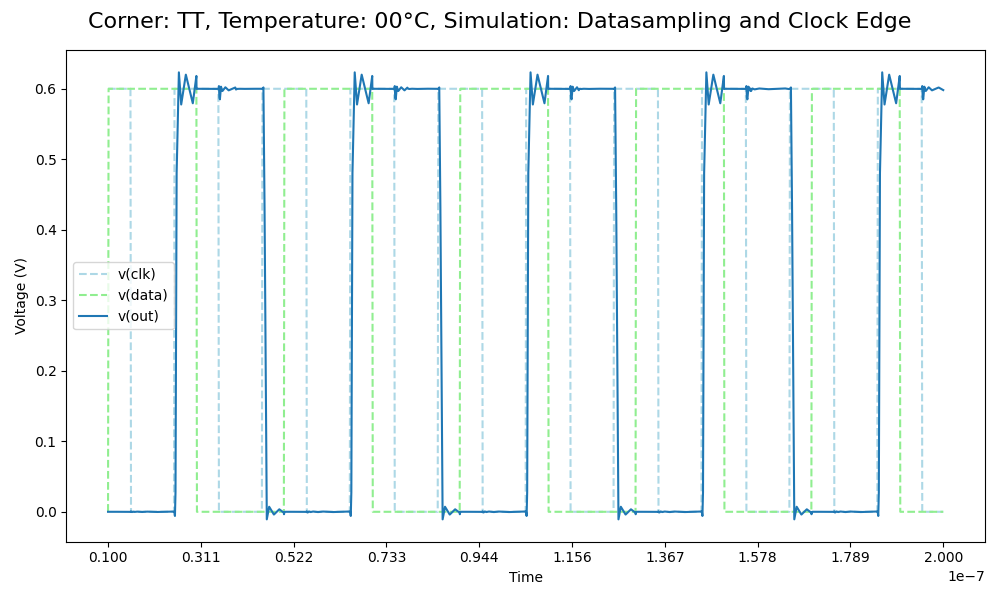
\includegraphics[height= 0.21\textheight]{figures/aimspice/0.600_0.1u_0.1u_0.3u_0.1u/functionality/TT00W1.png}
    \vspace{5pt}
    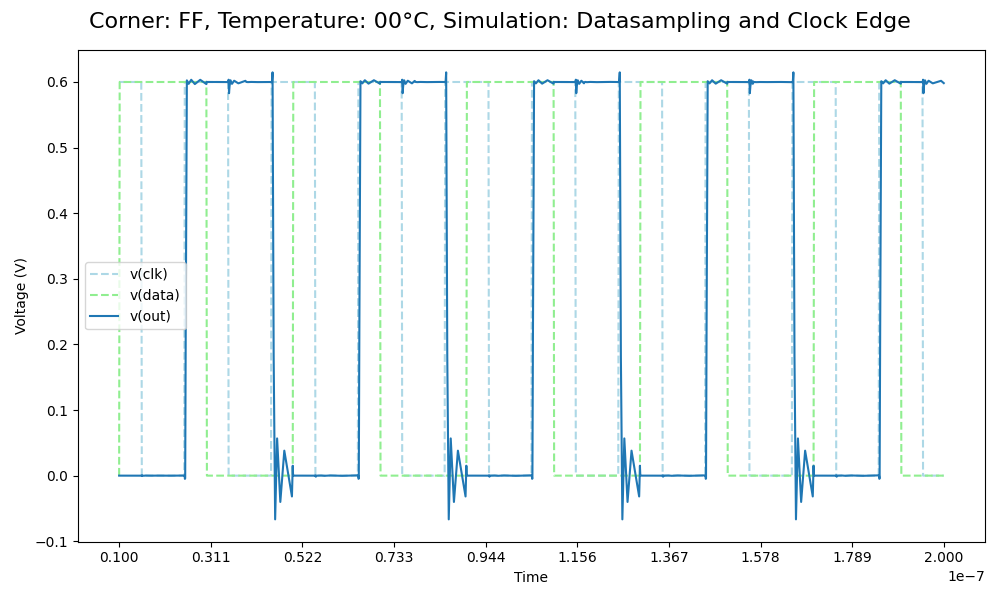
\includegraphics[height= 0.21\textheight]{figures/aimspice/0.600_0.1u_0.1u_0.3u_0.1u/functionality/FF00W1.png}
    \vspace{5pt}
    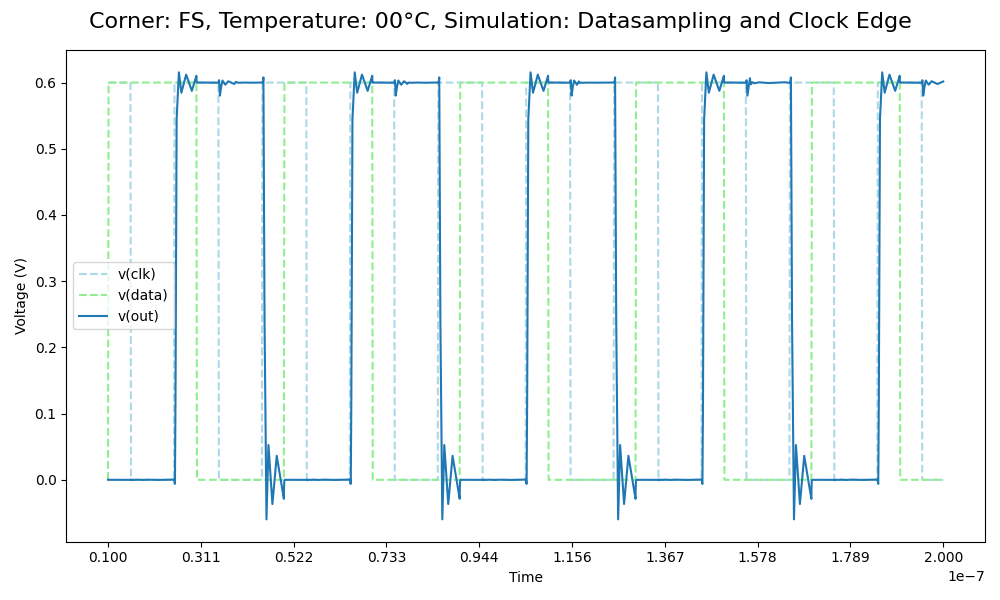
\includegraphics[height= 0.21\textheight]{figures/aimspice/0.600_0.1u_0.1u_0.3u_0.1u/functionality/FS00W1.png}
    \vspace{5pt}
    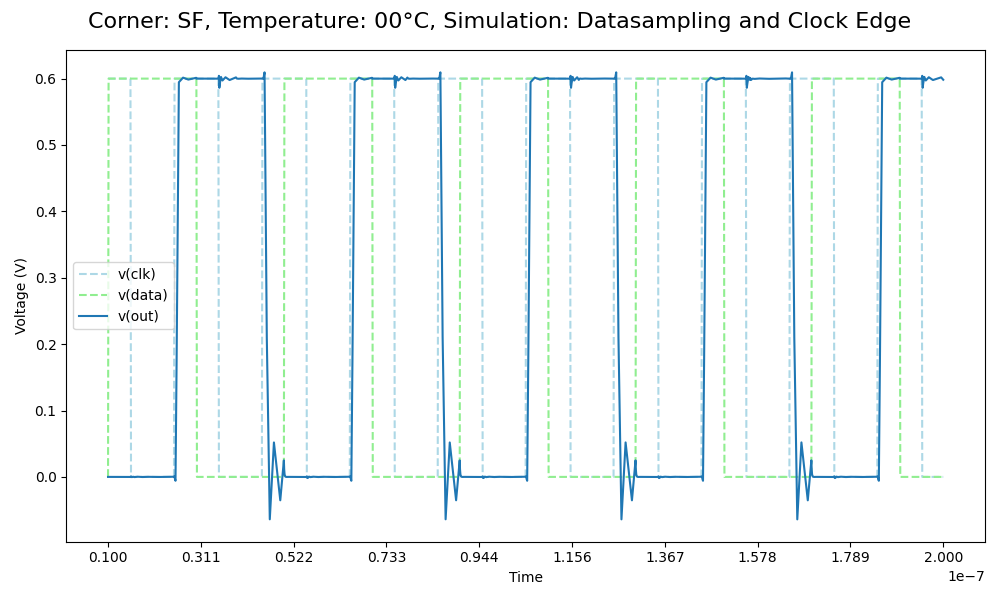
\includegraphics[height= 0.21\textheight]{figures/aimspice/0.600_0.1u_0.1u_0.3u_0.1u/functionality/SF00W1.png}
    \vspace{5pt}
    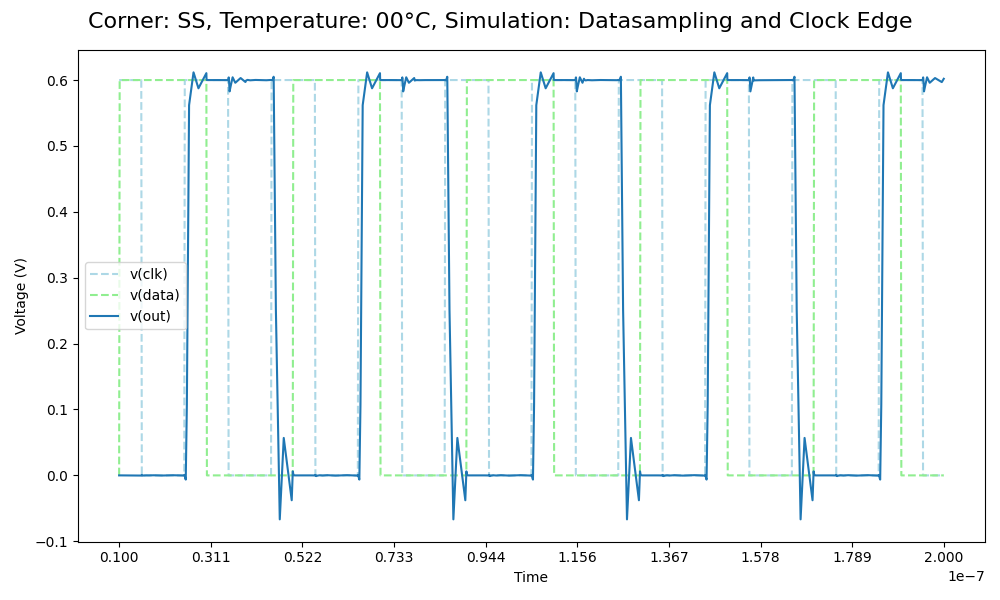
\includegraphics[height= 0.21\textheight]{figures/aimspice/0.600_0.1u_0.1u_0.3u_0.1u/functionality/SS00W1.png}
    \caption{Simulation of datasampling at clock edge at 0 degrees Celsius.}
    \label{fig:aimspice_W1_0}
\end{figure}

\pagebreak

\begin{figure}[H]
    \centering
    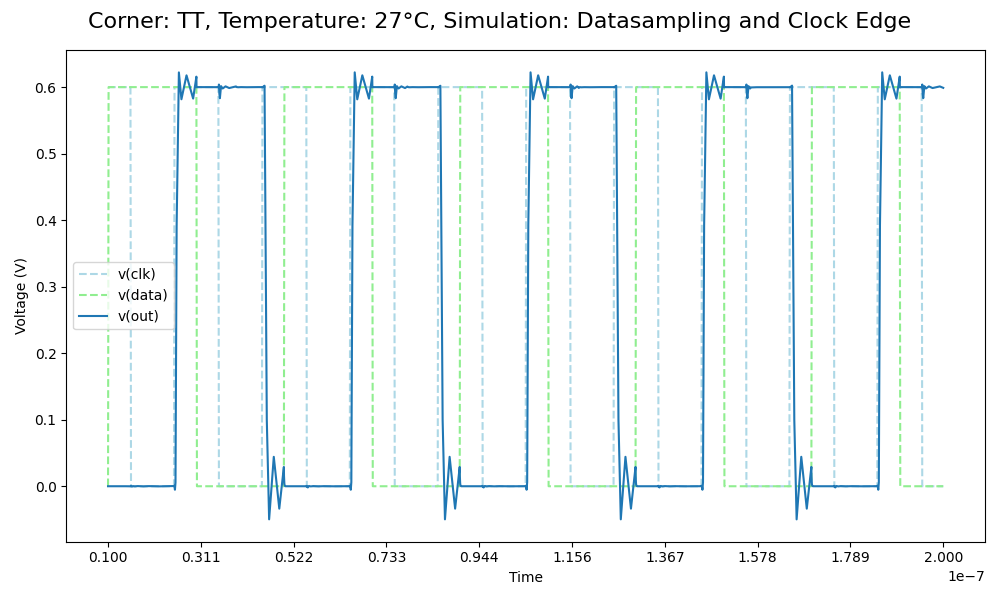
\includegraphics[height= 0.21\textheight]{figures/aimspice/0.600_0.1u_0.1u_0.3u_0.1u/functionality/TT27W1.png}
    \vspace{5pt}
    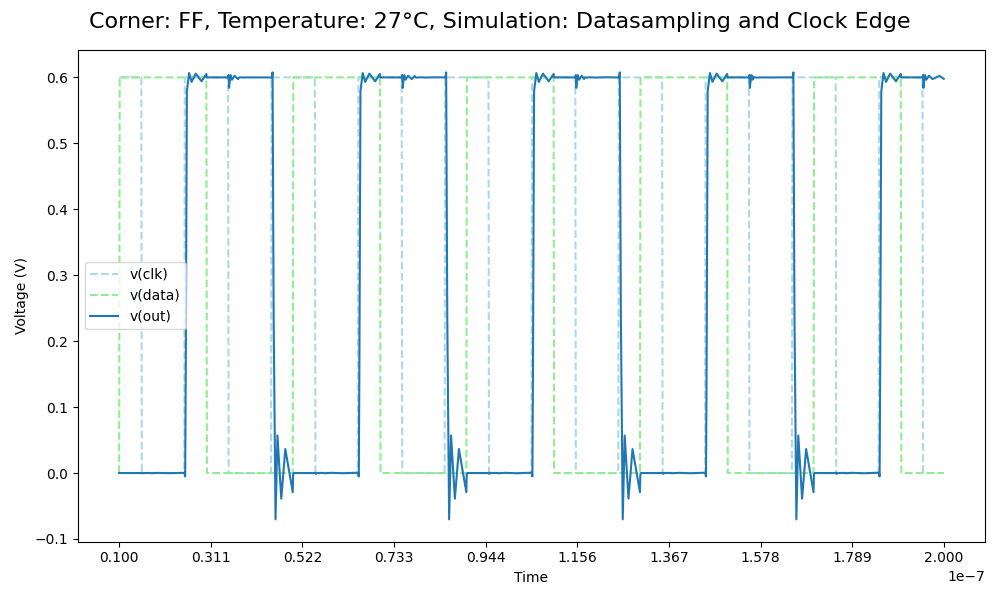
\includegraphics[height= 0.21\textheight]{figures/aimspice/0.600_0.1u_0.1u_0.3u_0.1u/functionality/FF27W1.png}
    \vspace{5pt}
    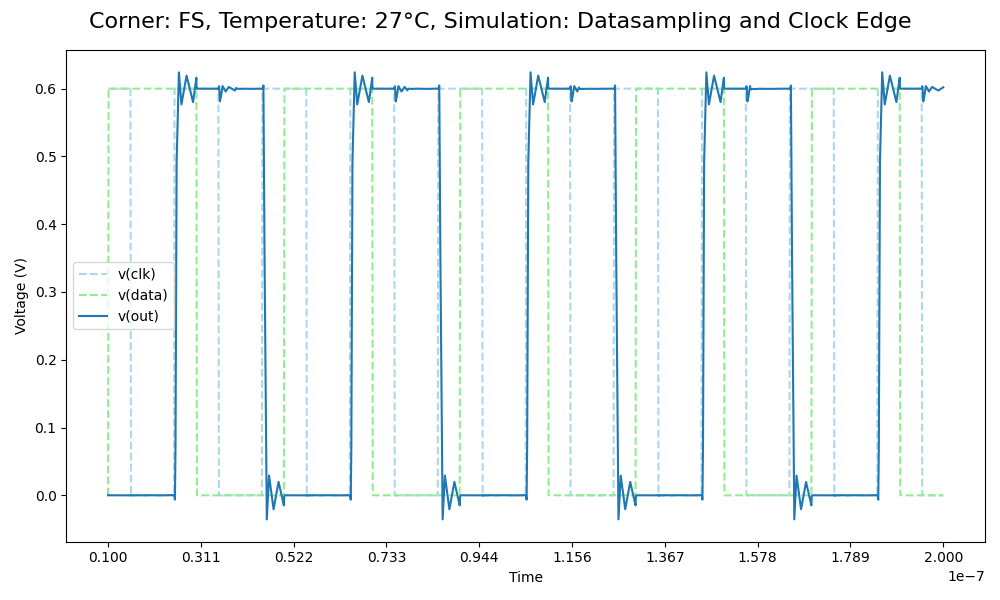
\includegraphics[height= 0.21\textheight]{figures/aimspice/0.600_0.1u_0.1u_0.3u_0.1u/functionality/FS27W1.png}
    \vspace{5pt}
    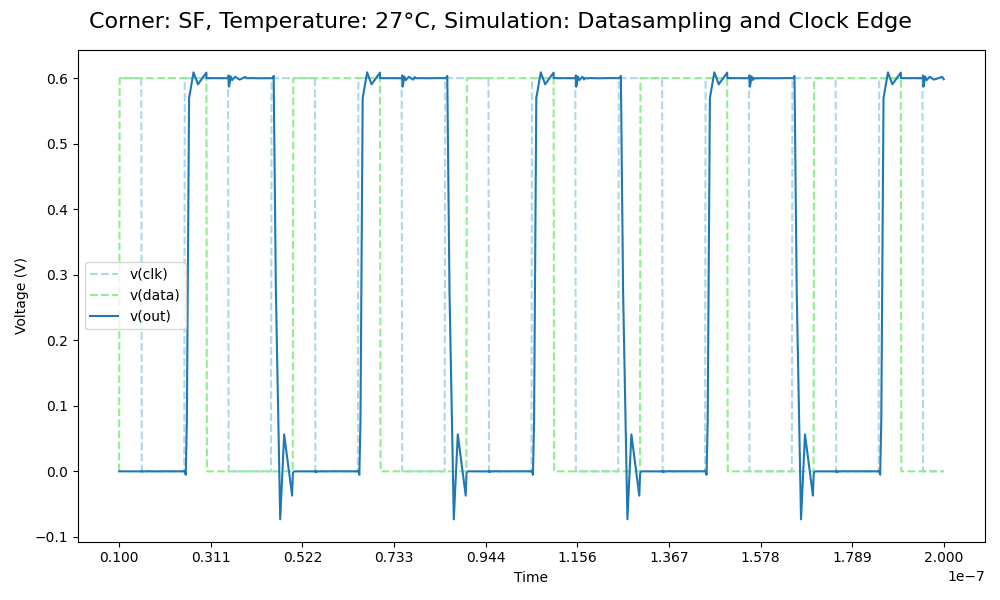
\includegraphics[height= 0.21\textheight]{figures/aimspice/0.600_0.1u_0.1u_0.3u_0.1u/functionality/SF27W1.png}
    \vspace{5pt}
    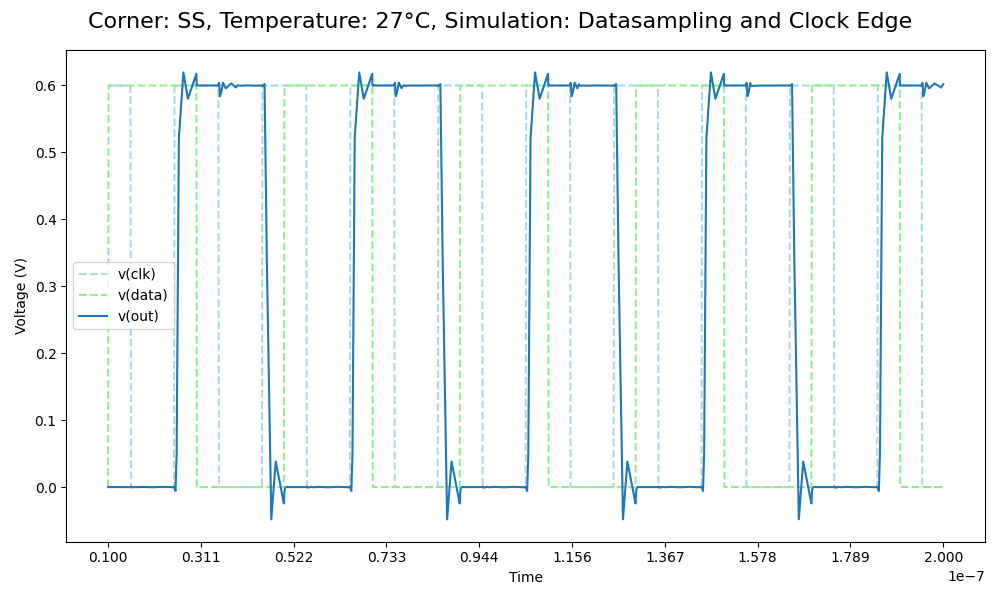
\includegraphics[height= 0.21\textheight]{figures/aimspice/0.600_0.1u_0.1u_0.3u_0.1u/functionality/SS27W1.png}
    \caption{Simulation of datasampling at clock edge at 27 degrees Celsius.}
    \label{fig:aimspice_W1_27}
\end{figure}

\pagebreak

\begin{figure}[H]
    \centering
    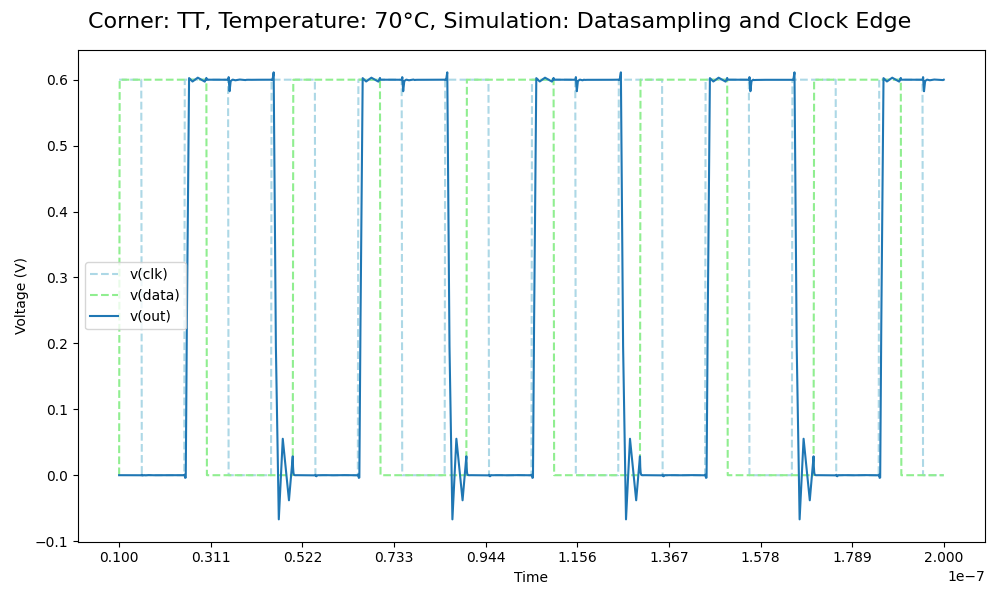
\includegraphics[height= 0.21\textheight]{figures/aimspice/0.600_0.1u_0.1u_0.3u_0.1u/functionality/TT70W1.png}
    \vspace{5pt}
    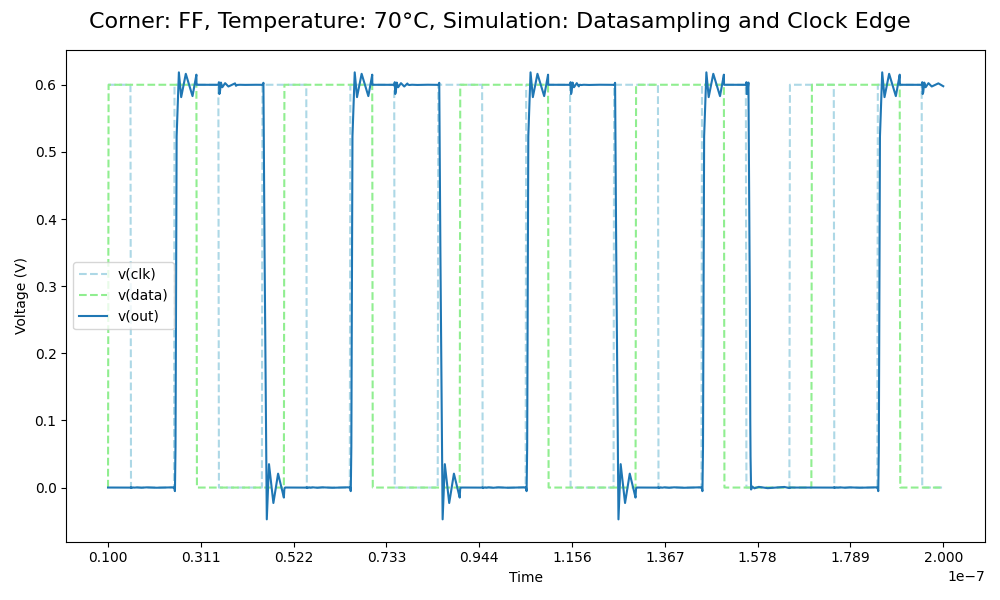
\includegraphics[height= 0.21\textheight]{figures/aimspice/0.600_0.1u_0.1u_0.3u_0.1u/functionality/FF70W1.png}
    \vspace{5pt}
    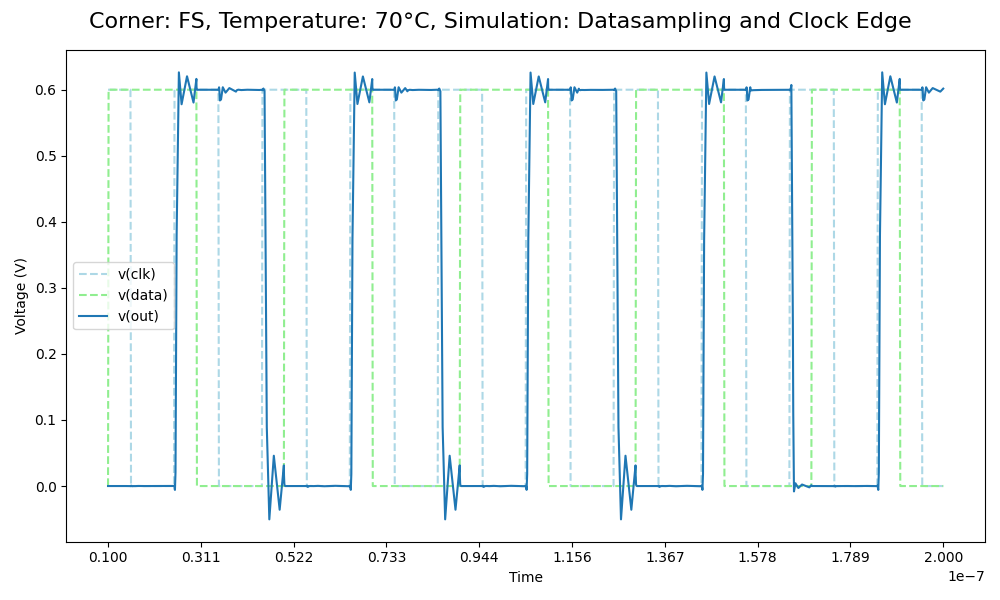
\includegraphics[height= 0.21\textheight]{figures/aimspice/0.600_0.1u_0.1u_0.3u_0.1u/functionality/FS70W1.png}
    \vspace{5pt}
    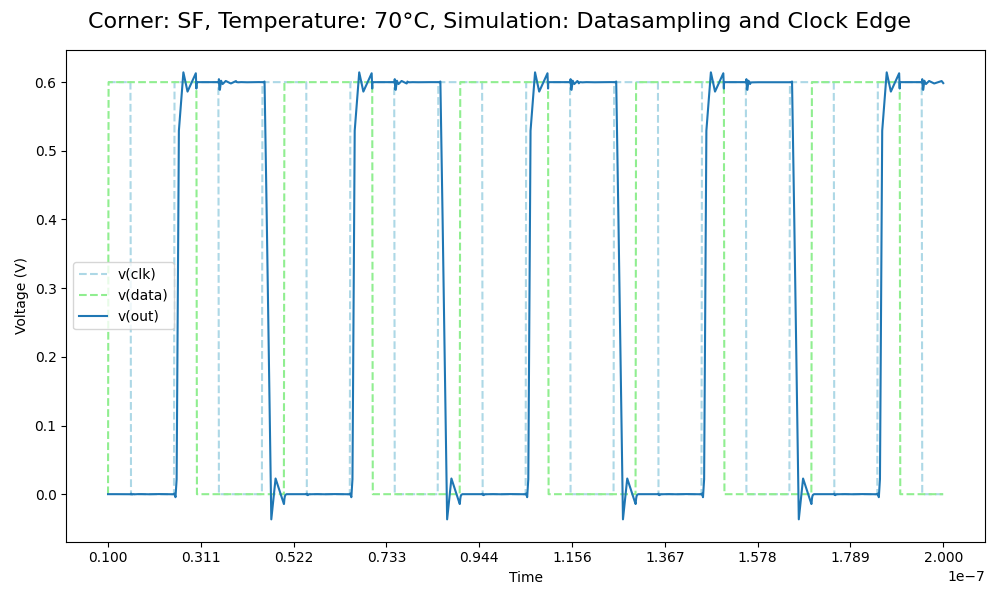
\includegraphics[height= 0.21\textheight]{figures/aimspice/0.600_0.1u_0.1u_0.3u_0.1u/functionality/SF70W1.png}
    \vspace{5pt}
    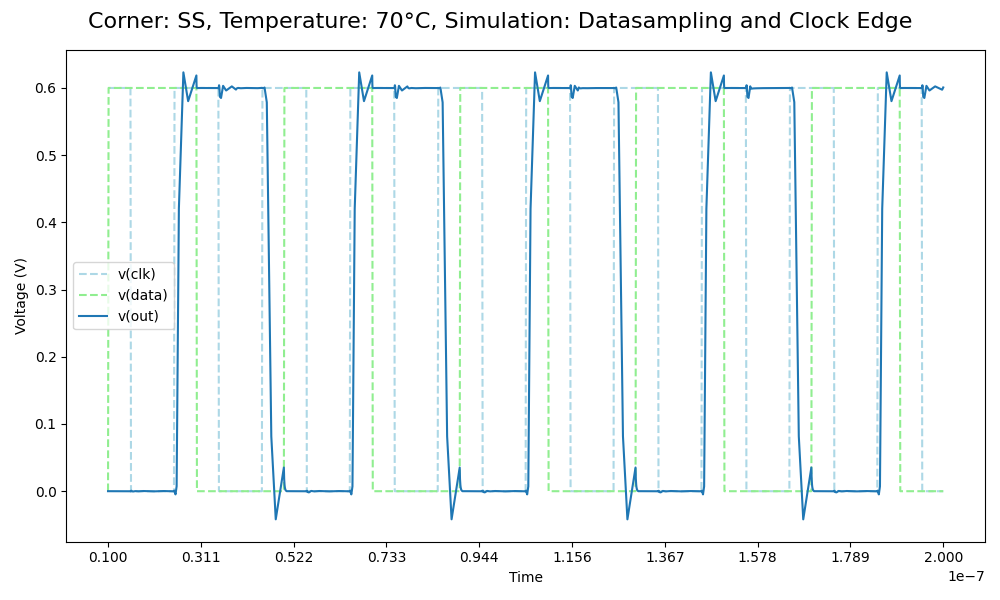
\includegraphics[height= 0.21\textheight]{figures/aimspice/0.600_0.1u_0.1u_0.3u_0.1u/functionality/SS70W1.png}
    \caption{Simulation of datasampling at clock edge at 70 degrees Celsius.}
    \label{fig:aimspice_W1_70}
\end{figure}

\pagebreak

\begin{figure}[H]
    \centering
    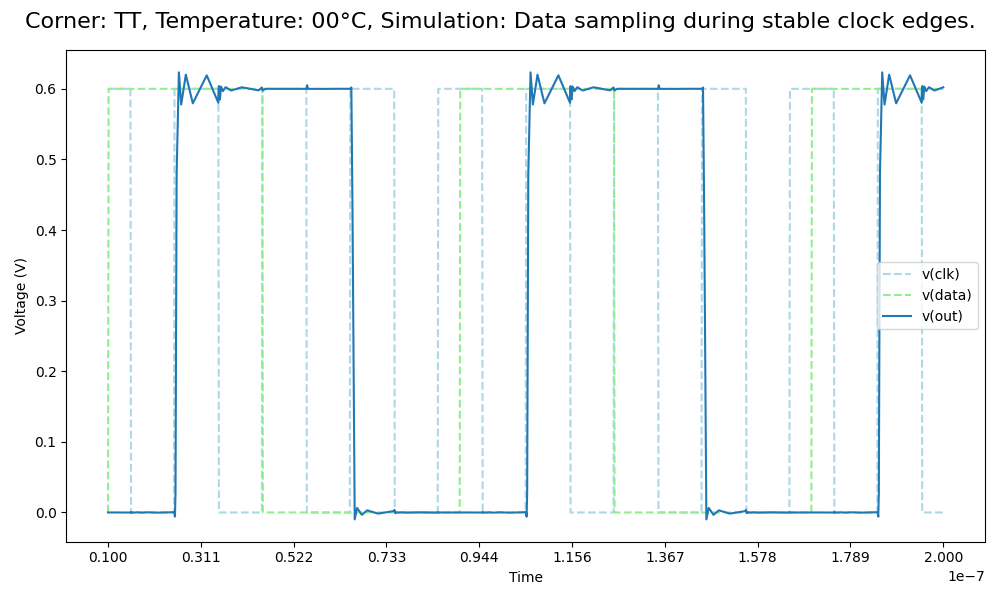
\includegraphics[height= 0.21\textheight]{figures/aimspice/0.600_0.1u_0.1u_0.3u_0.1u/functionality/TT00W2.png}
    \vspace{5pt}
    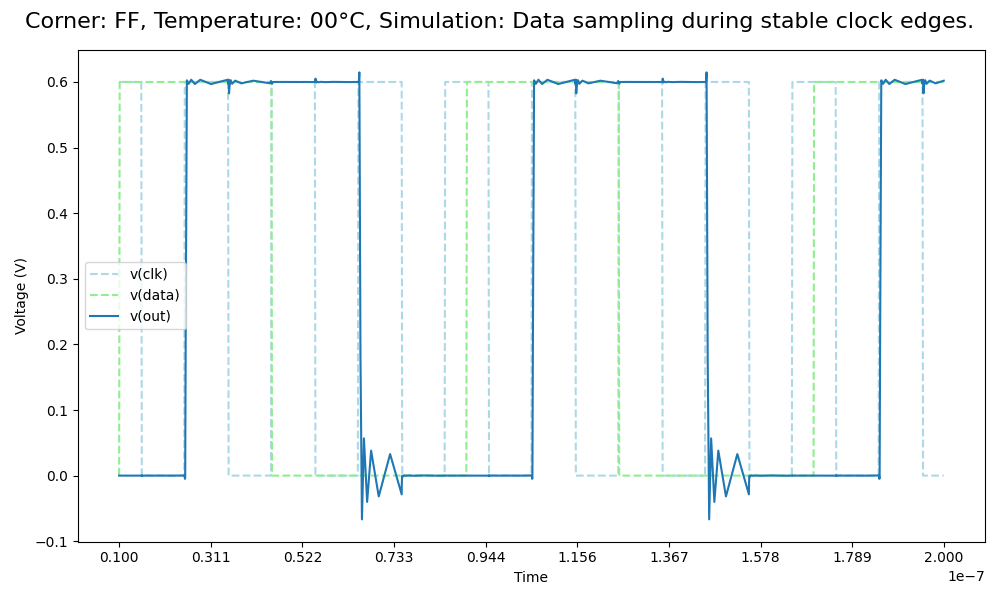
\includegraphics[height= 0.21\textheight]{figures/aimspice/0.600_0.1u_0.1u_0.3u_0.1u/functionality/FF00W2.png}
    \vspace{5pt}
    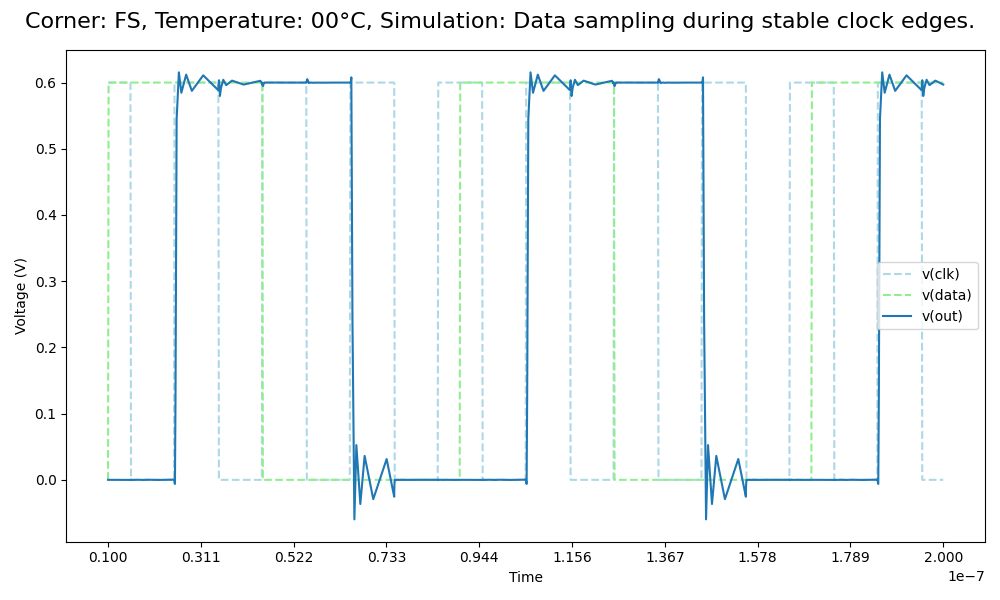
\includegraphics[height= 0.21\textheight]{figures/aimspice/0.600_0.1u_0.1u_0.3u_0.1u/functionality/FS00W2.png}
    \vspace{5pt}
    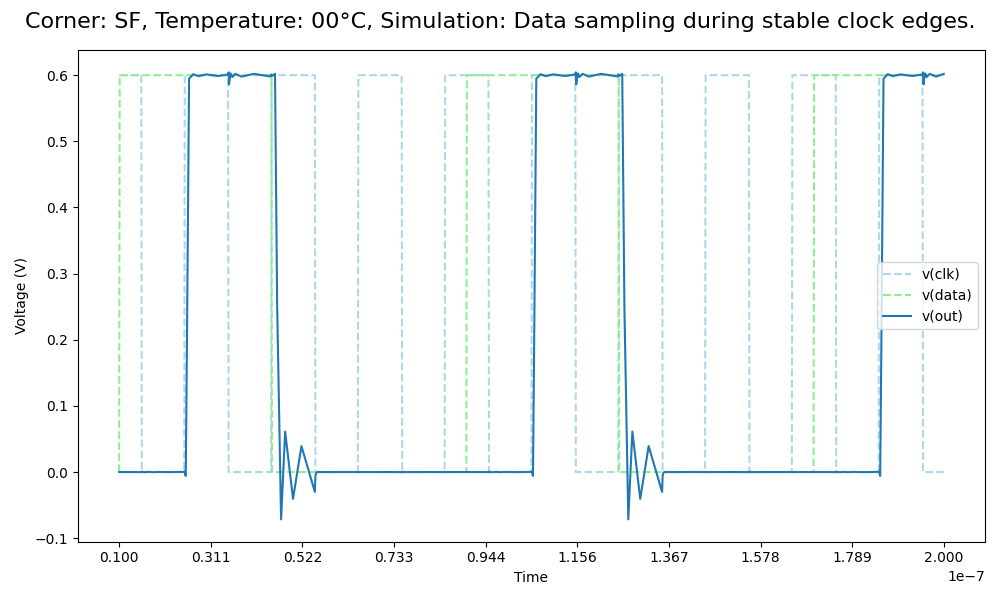
\includegraphics[height= 0.21\textheight]{figures/aimspice/0.600_0.1u_0.1u_0.3u_0.1u/functionality/SF00W2.png}
    \vspace{5pt}
    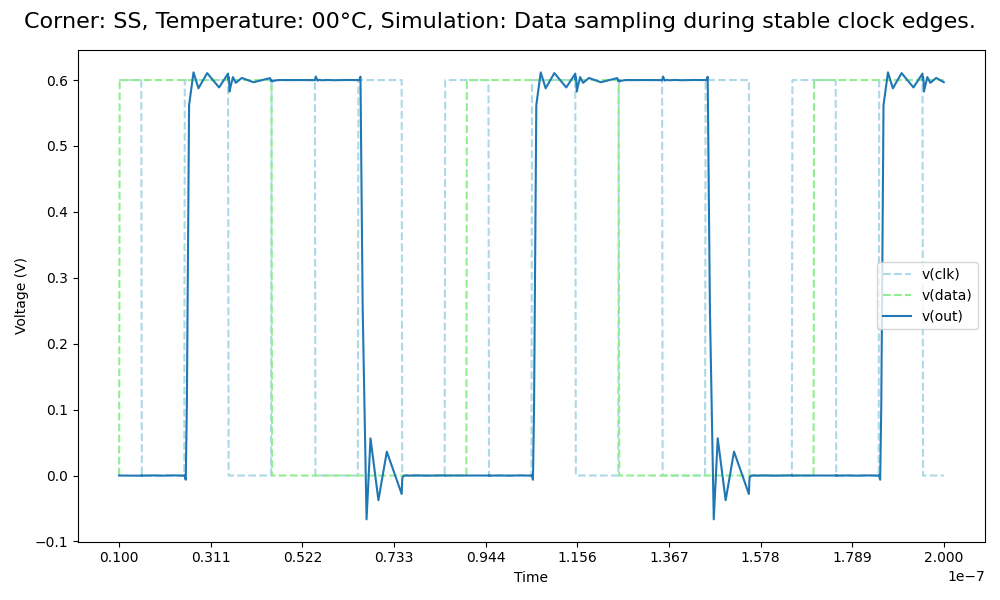
\includegraphics[height= 0.21\textheight]{figures/aimspice/0.600_0.1u_0.1u_0.3u_0.1u/functionality/SS00W2.png}
    \caption{Simulation of datasampling when the data stays the same for a few clock edges at 0 degrees celcius.}
    \label{fig:aimspice_W2_0}
\end{figure}

\pagebreak

\begin{figure}[H]
    \centering
    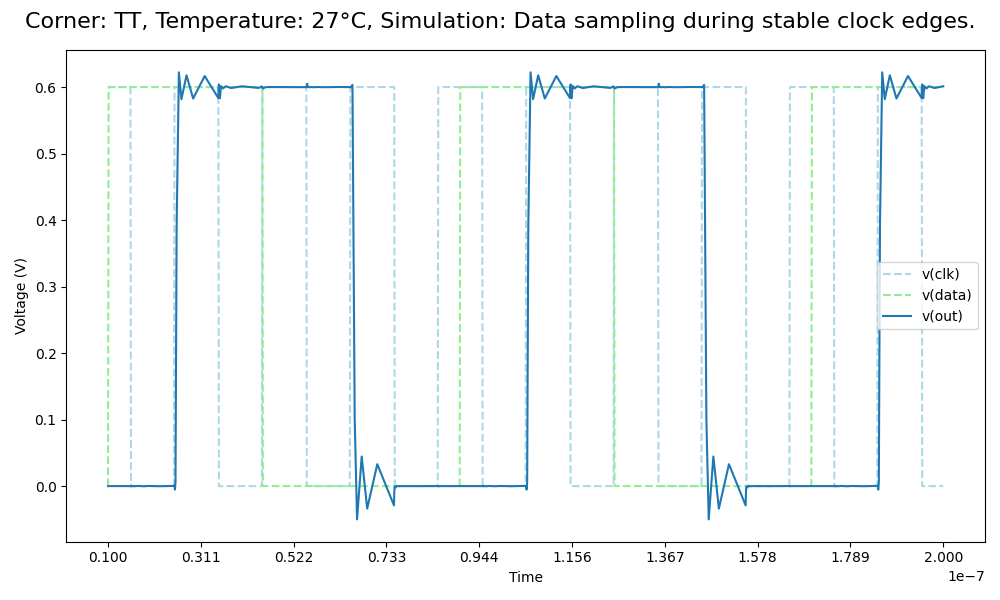
\includegraphics[height= 0.21\textheight]{figures/aimspice/0.600_0.1u_0.1u_0.3u_0.1u/functionality/TT27W2.png}
    \vspace{5pt}
    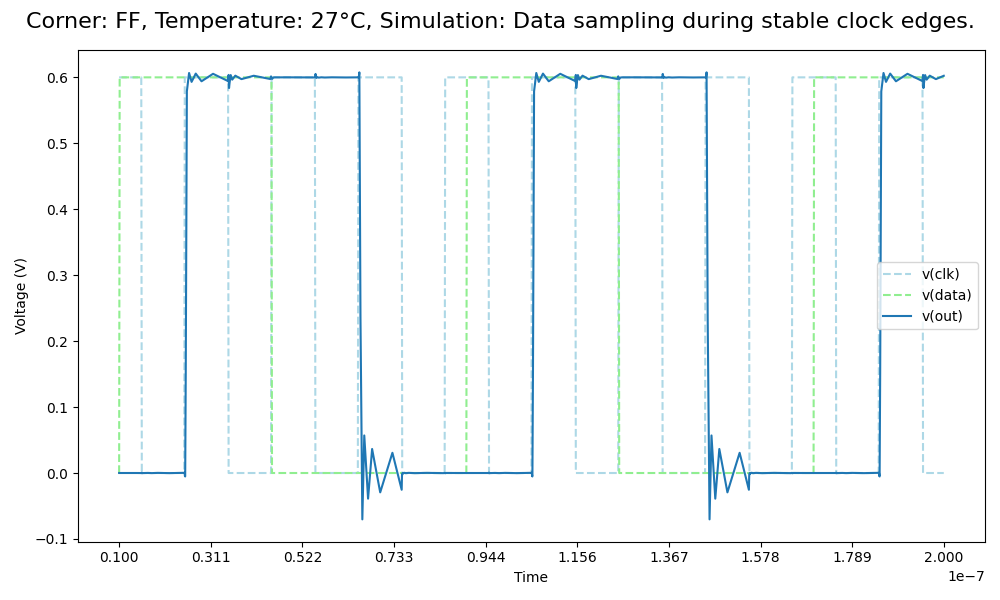
\includegraphics[height= 0.21\textheight]{figures/aimspice/0.600_0.1u_0.1u_0.3u_0.1u/functionality/FF27W2.png}
    \vspace{5pt}
    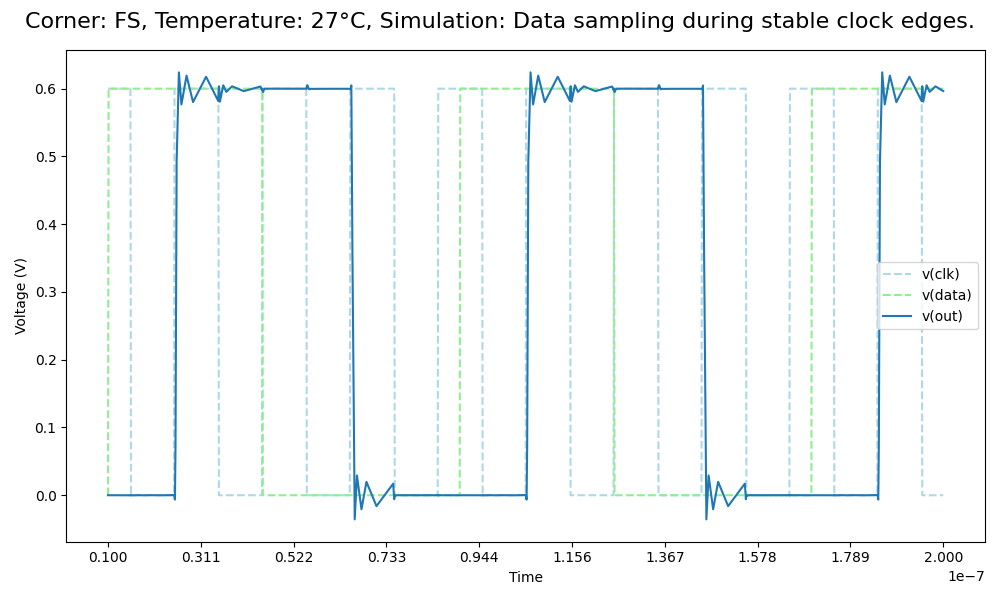
\includegraphics[height= 0.21\textheight]{figures/aimspice/0.600_0.1u_0.1u_0.3u_0.1u/functionality/FS27W2.png}
    \vspace{5pt}
    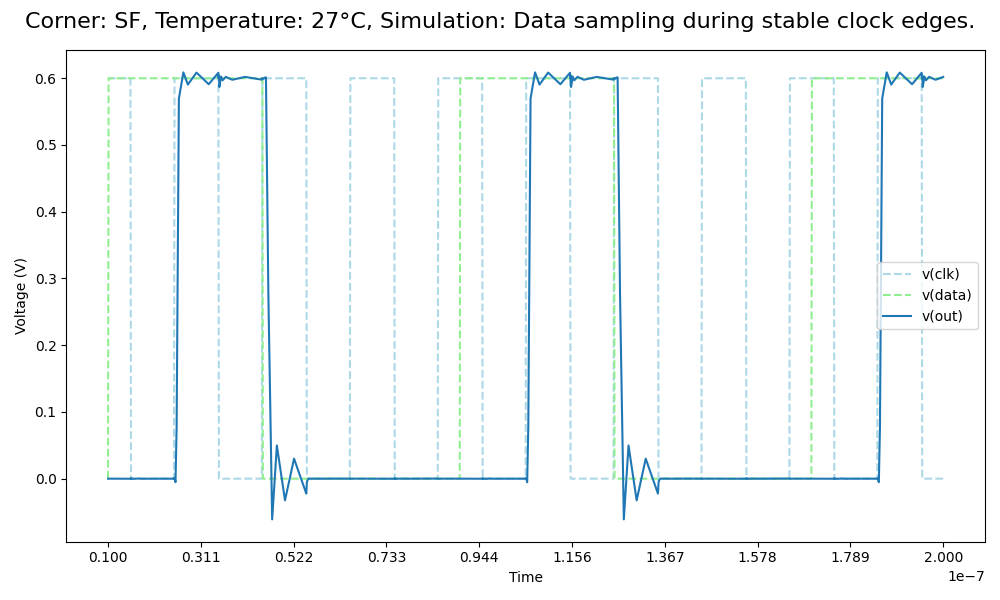
\includegraphics[height= 0.21\textheight]{figures/aimspice/0.600_0.1u_0.1u_0.3u_0.1u/functionality/SF27W2.png}
    \vspace{5pt}
    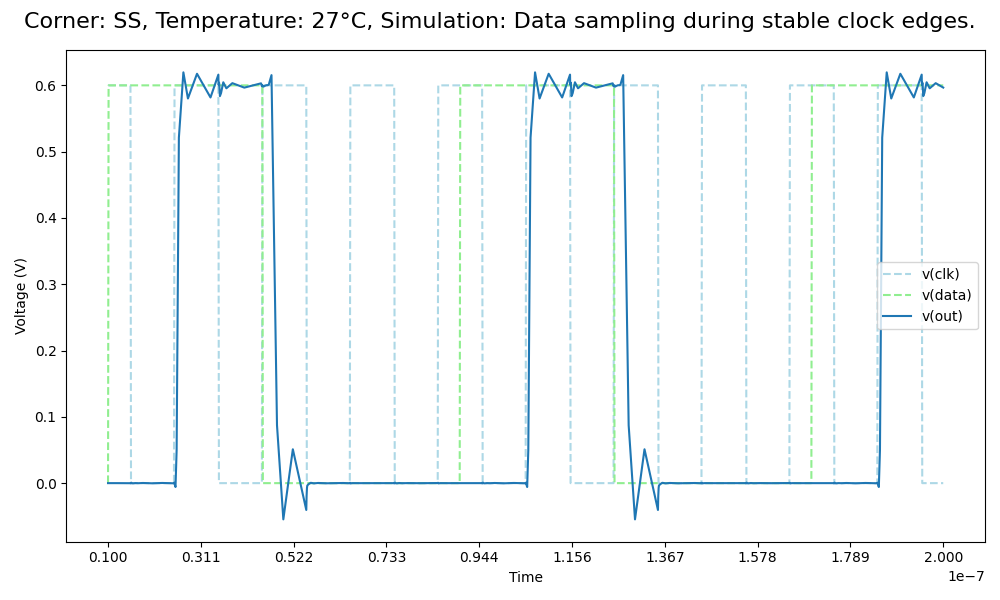
\includegraphics[height= 0.21\textheight]{figures/aimspice/0.600_0.1u_0.1u_0.3u_0.1u/functionality/SS27W2.png}
    \caption{Simulation of datasampling when the data stays the same for a few clock edges at 27 degrees celcius.}
    \label{fig:aimspice_W2_27}
\end{figure}

\pagebreak

\begin{figure}[H]
    \centering
    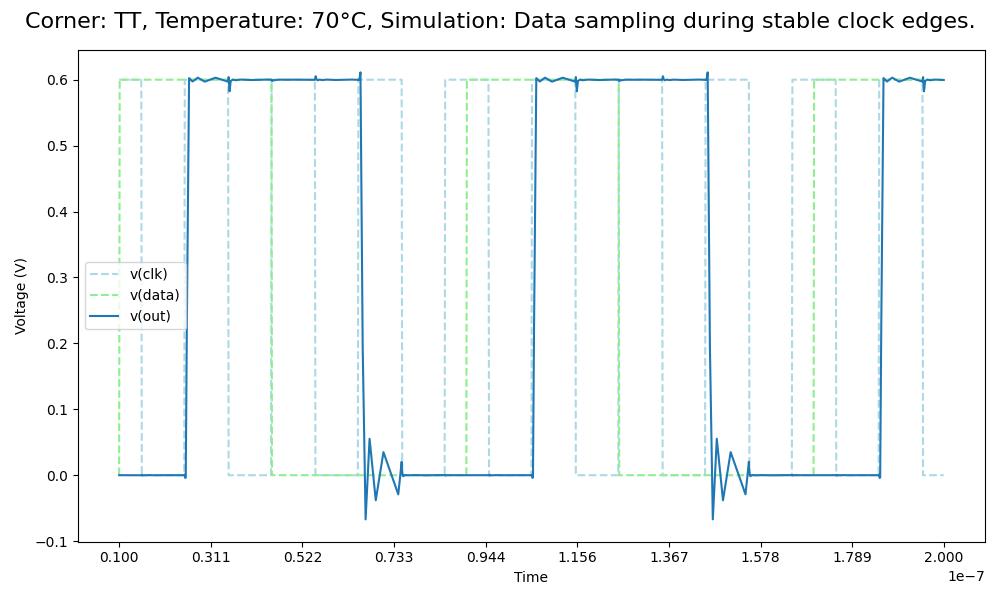
\includegraphics[height= 0.21\textheight]{figures/aimspice/0.600_0.1u_0.1u_0.3u_0.1u/functionality/TT70W2.png}
    \vspace{5pt}
    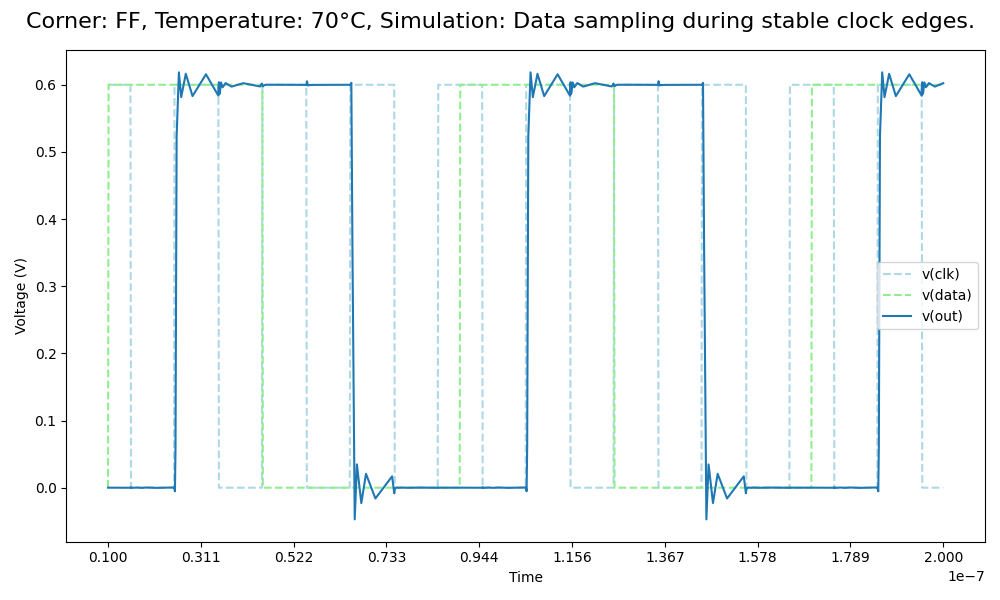
\includegraphics[height= 0.21\textheight]{figures/aimspice/0.600_0.1u_0.1u_0.3u_0.1u/functionality/FF70W2.png}
    \vspace{5pt}
    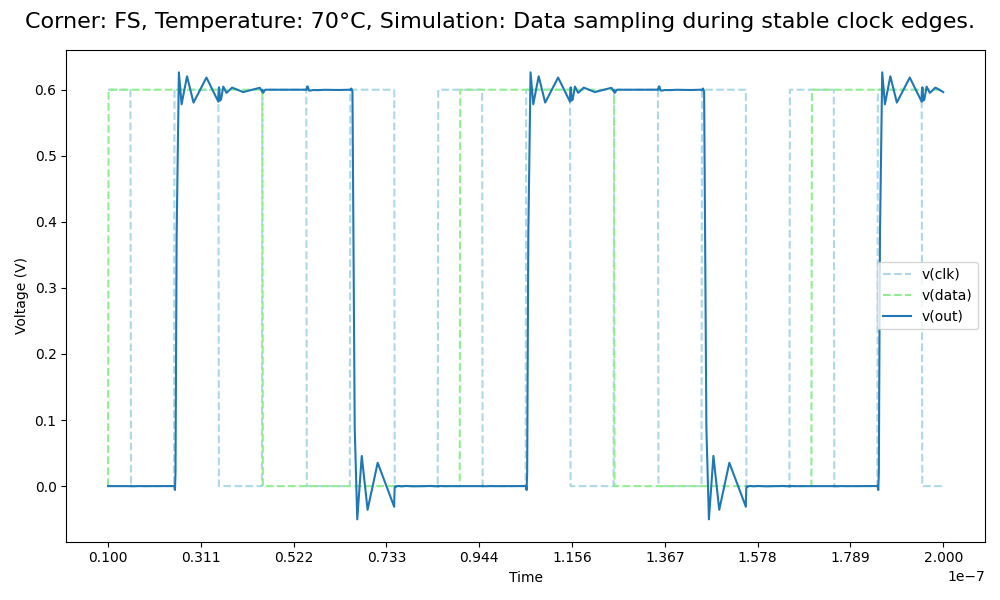
\includegraphics[height= 0.21\textheight]{figures/aimspice/0.600_0.1u_0.1u_0.3u_0.1u/functionality/FS70W2.png}
    \vspace{5pt}
    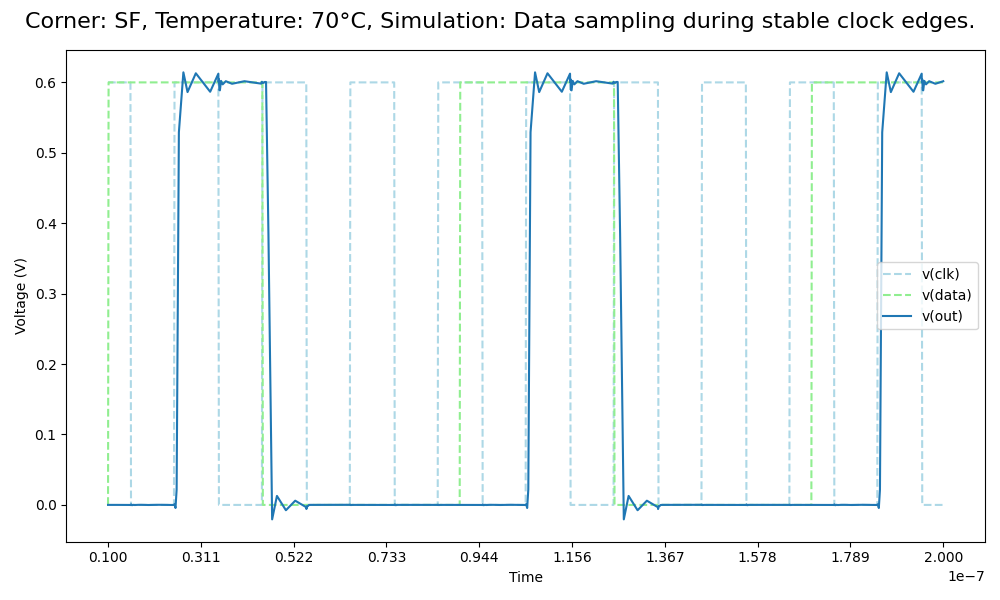
\includegraphics[height= 0.21\textheight]{figures/aimspice/0.600_0.1u_0.1u_0.3u_0.1u/functionality/SF70W2.png}
    \vspace{5pt}
    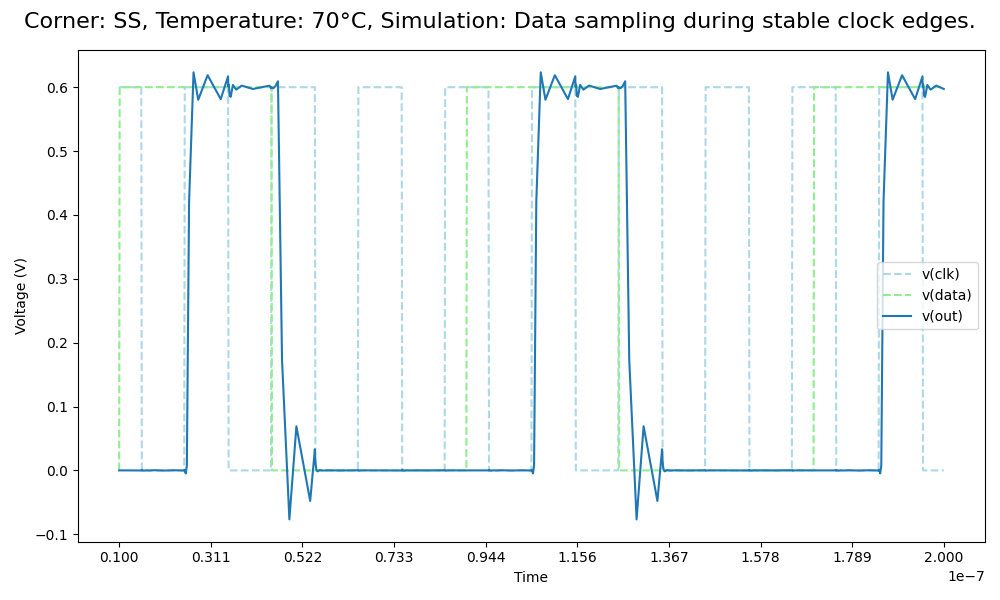
\includegraphics[height= 0.21\textheight]{figures/aimspice/0.600_0.1u_0.1u_0.3u_0.1u/functionality/SS70W2.png}
    \caption{Simulation of datasampling when the data stays the same for a few clock edges at 70 degrees celcius.}
    \label{fig:aimspice_W2_70}
\end{figure}

\pagebreak

\pagebreak

\begin{figure}[H]
    \centering
    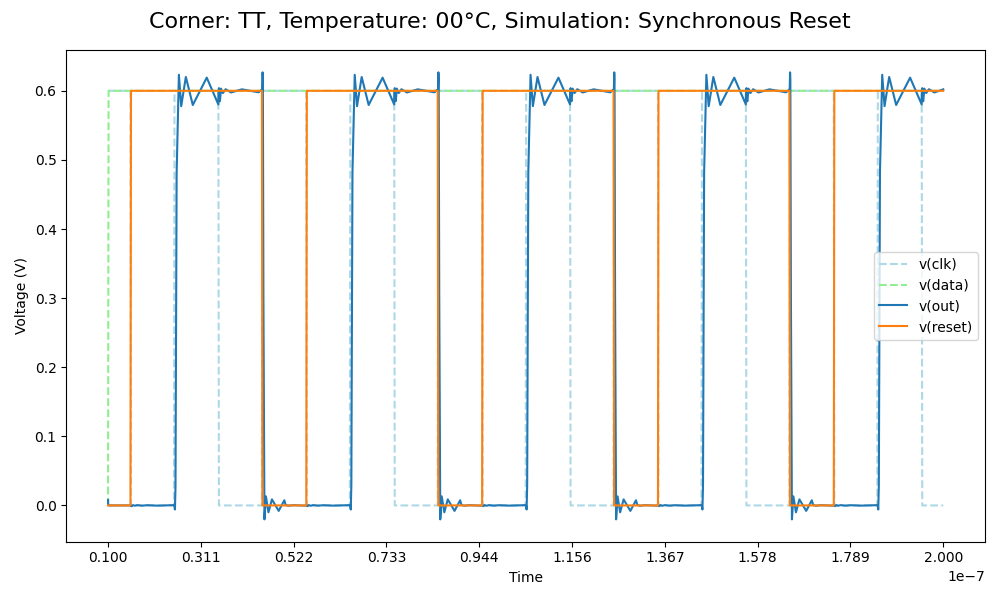
\includegraphics[height= 0.21\textheight]{figures/aimspice/0.600_0.1u_0.1u_0.3u_0.1u/functionality/TT00W3.png}
    \vspace{5pt}
    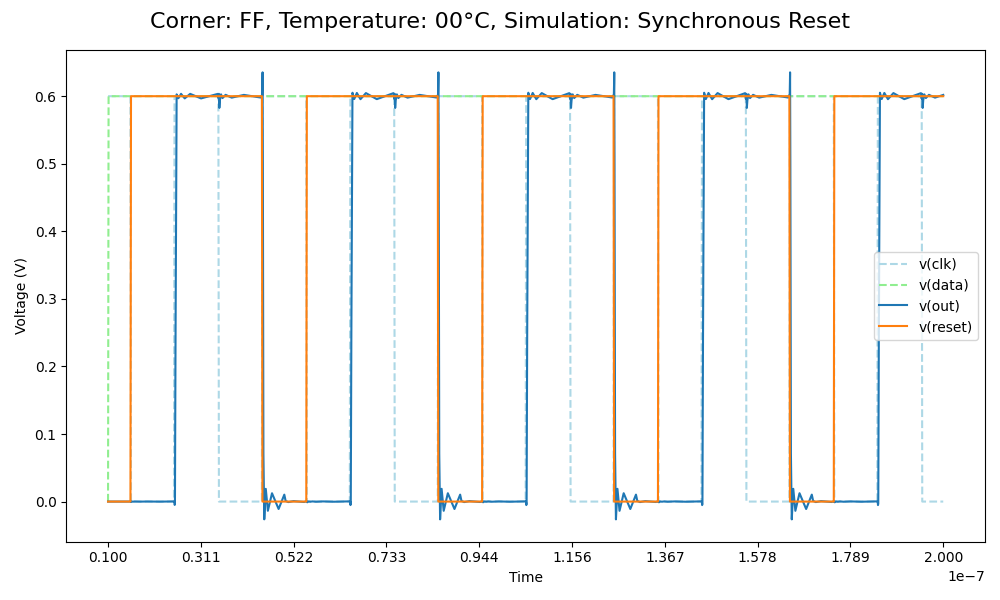
\includegraphics[height= 0.21\textheight]{figures/aimspice/0.600_0.1u_0.1u_0.3u_0.1u/functionality/FF00W3.png}
    \vspace{5pt}
    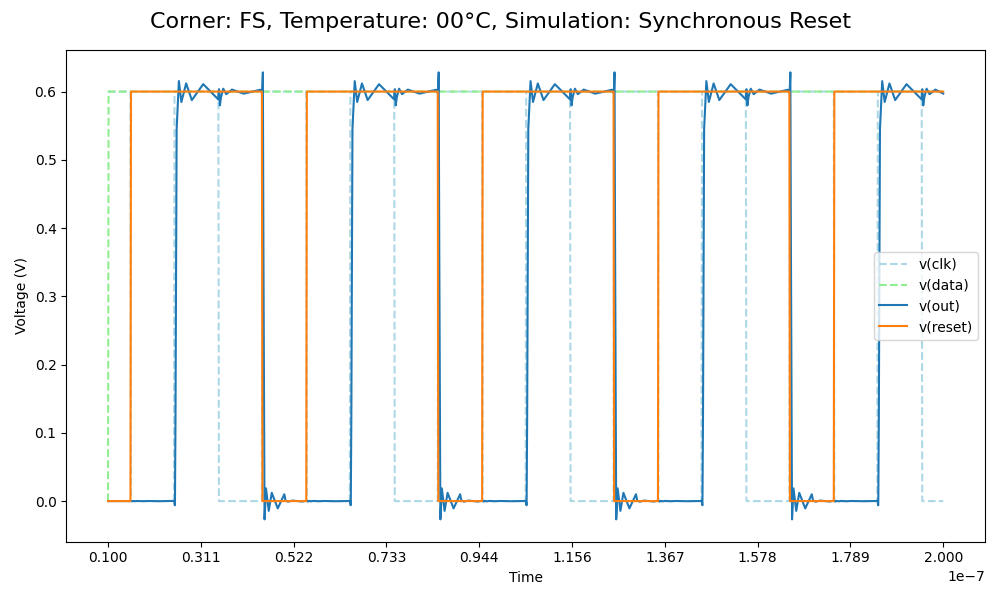
\includegraphics[height= 0.21\textheight]{figures/aimspice/0.600_0.1u_0.1u_0.3u_0.1u/functionality/FS00W3.png}
    \vspace{5pt}
    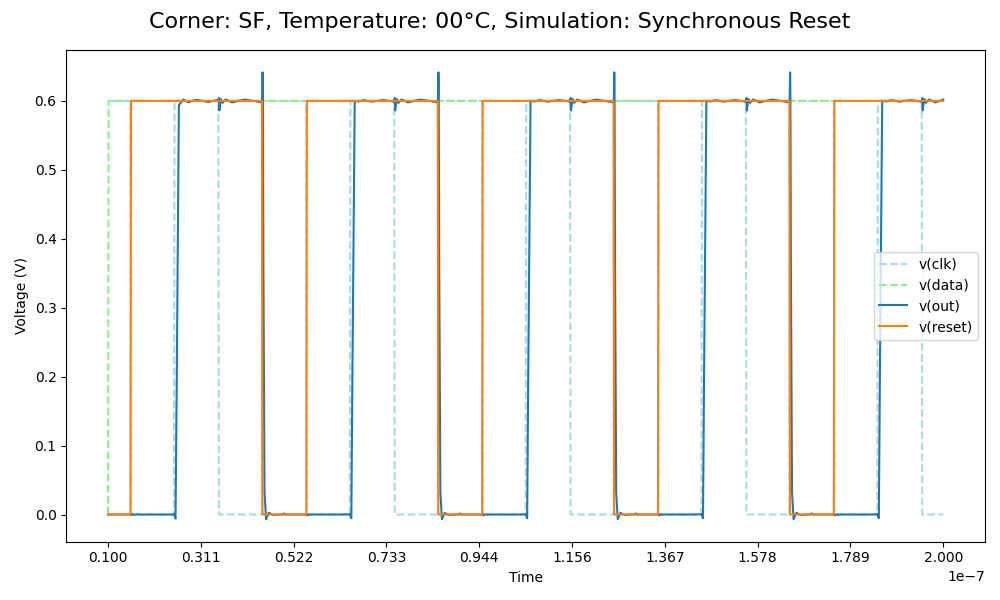
\includegraphics[height= 0.21\textheight]{figures/aimspice/0.600_0.1u_0.1u_0.3u_0.1u/functionality/SF00W3.png}
    \vspace{5pt}
    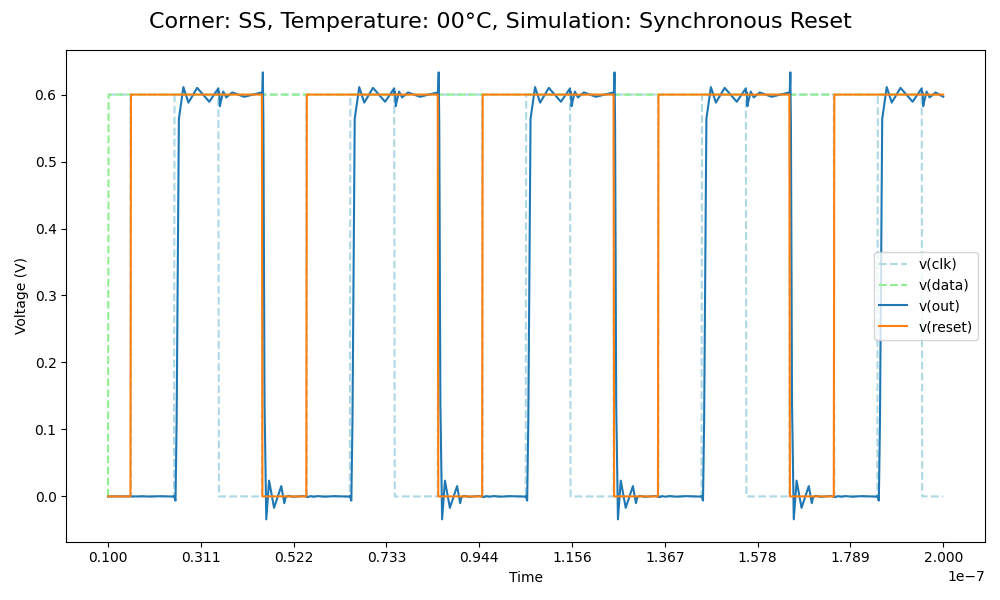
\includegraphics[height= 0.21\textheight]{figures/aimspice/0.600_0.1u_0.1u_0.3u_0.1u/functionality/SS00W3.png}
    \caption{Simulation of the reset at 0 degrees celcius.}
    \label{fig:aimspice_W3_0}
\end{figure}

\pagebreak

\begin{figure}[H]
    \centering
    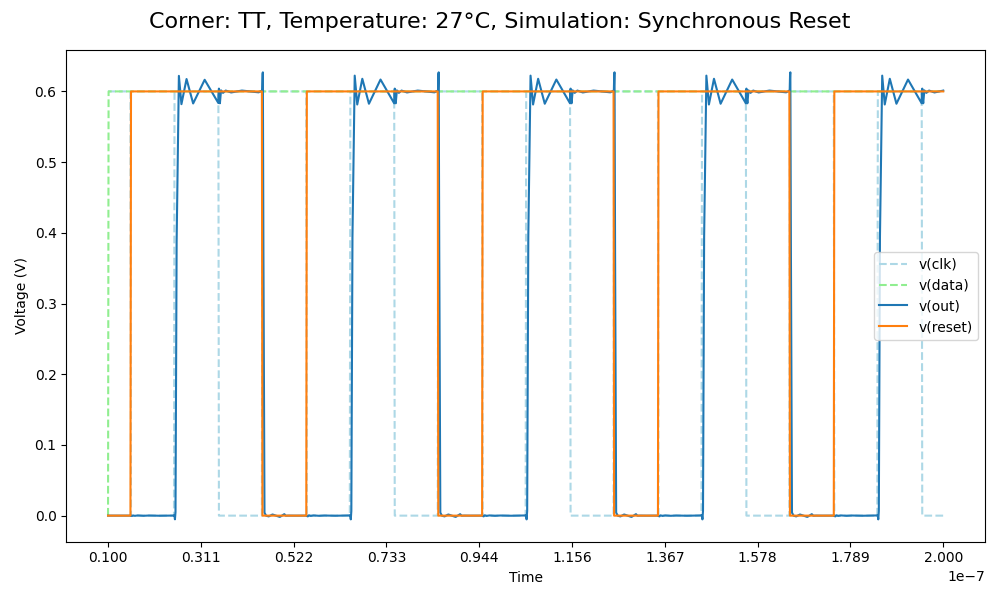
\includegraphics[height= 0.21\textheight]{figures/aimspice/0.600_0.1u_0.1u_0.3u_0.1u/functionality/TT27W3.png}
    \vspace{5pt}
    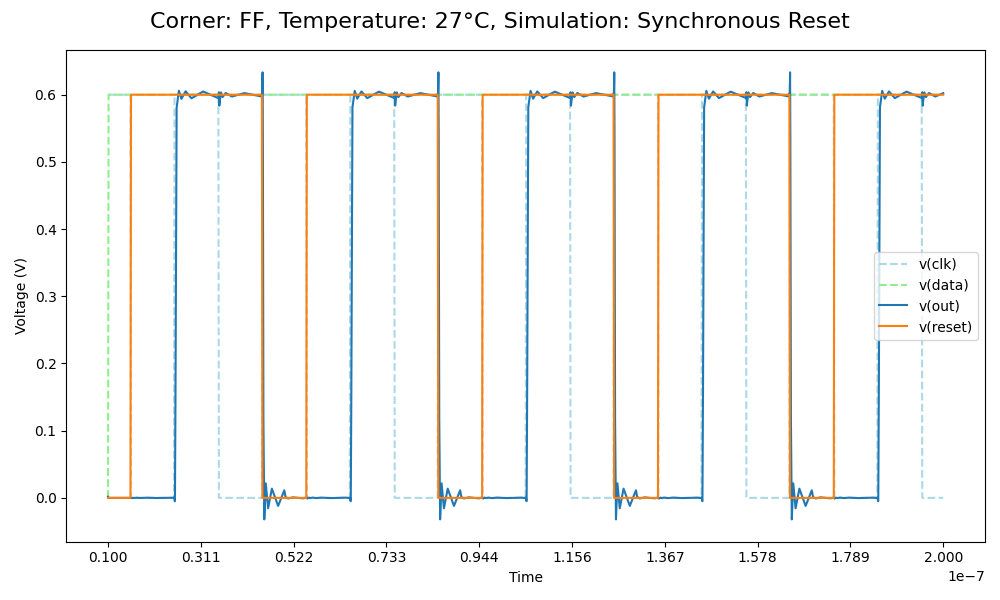
\includegraphics[height= 0.21\textheight]{figures/aimspice/0.600_0.1u_0.1u_0.3u_0.1u/functionality/FF27W3.png}
    \vspace{5pt}
    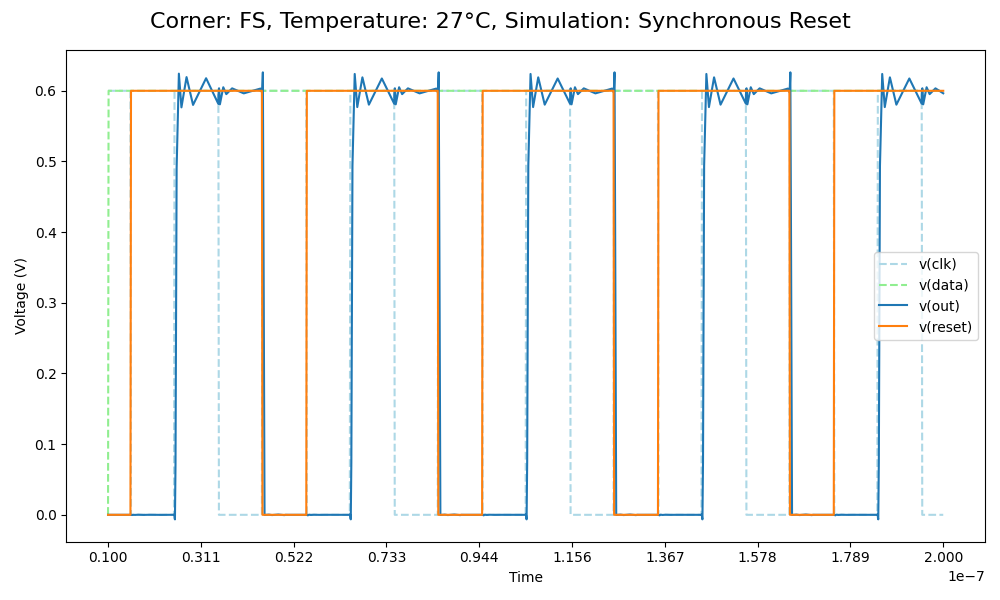
\includegraphics[height= 0.21\textheight]{figures/aimspice/0.600_0.1u_0.1u_0.3u_0.1u/functionality/FS27W3.png}
    \vspace{5pt}
    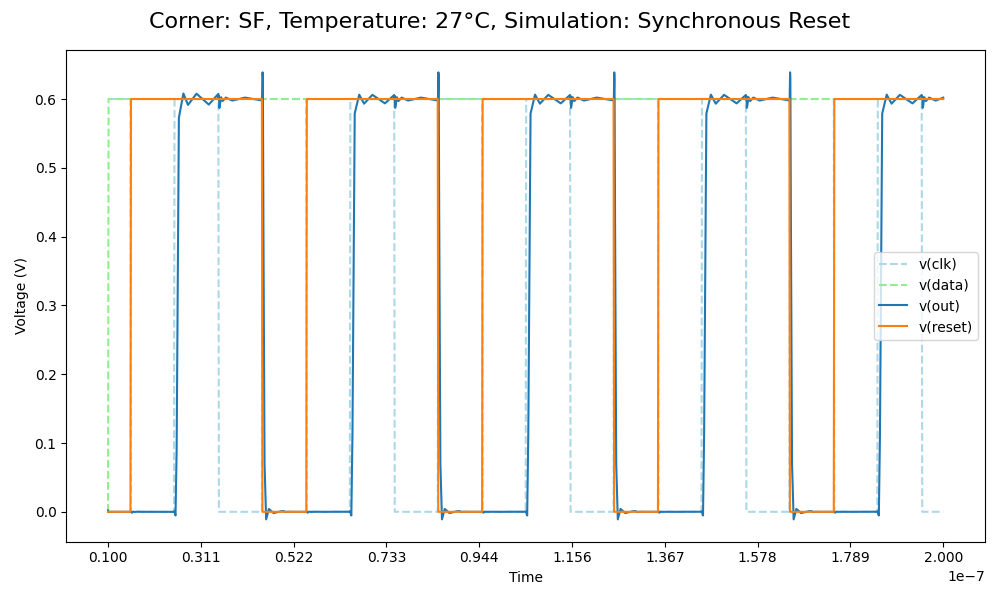
\includegraphics[height= 0.21\textheight]{figures/aimspice/0.600_0.1u_0.1u_0.3u_0.1u/functionality/SF27W3.png}
    \vspace{5pt}
    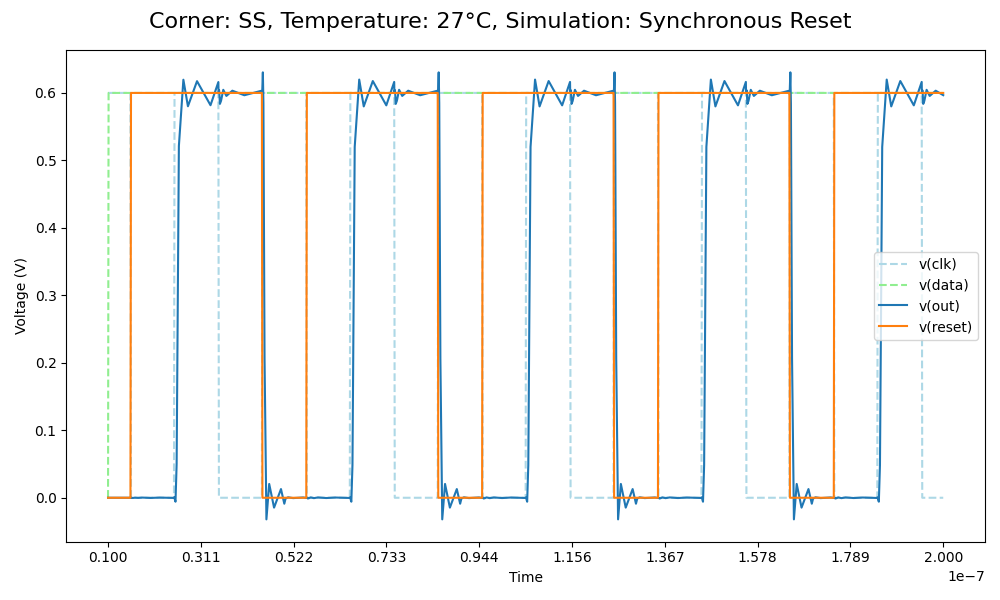
\includegraphics[height= 0.21\textheight]{figures/aimspice/0.600_0.1u_0.1u_0.3u_0.1u/functionality/SS27W3.png}
    \caption{Simulation of the reset at 27 degrees celcius.}
    \label{fig:aimspice_W3_27}
\end{figure}

\pagebreak

\begin{figure}[H]
    \centering
    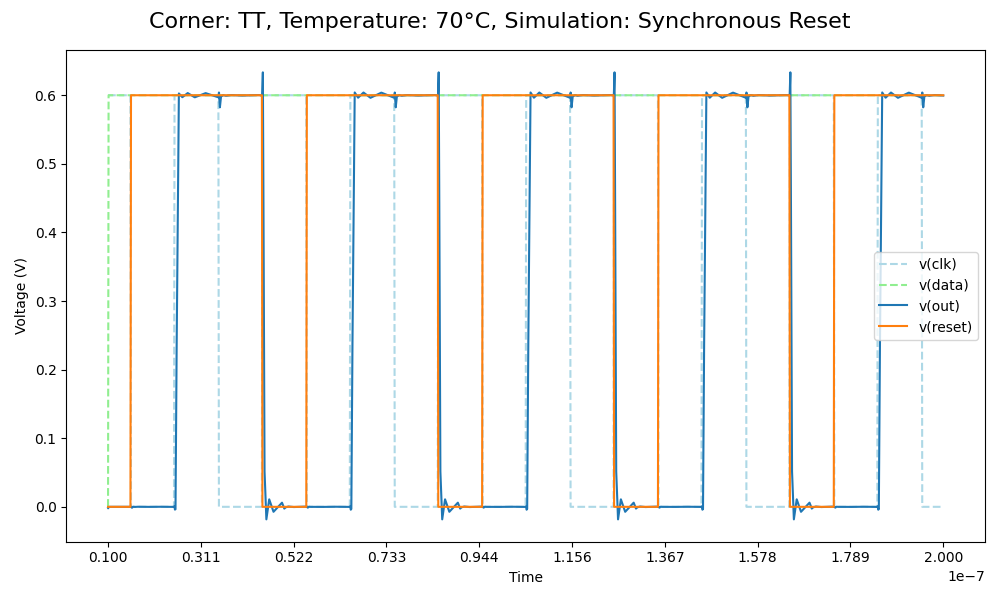
\includegraphics[height= 0.21\textheight]{figures/aimspice/0.600_0.1u_0.1u_0.3u_0.1u/functionality/TT70W3.png}
    \vspace{5pt}
    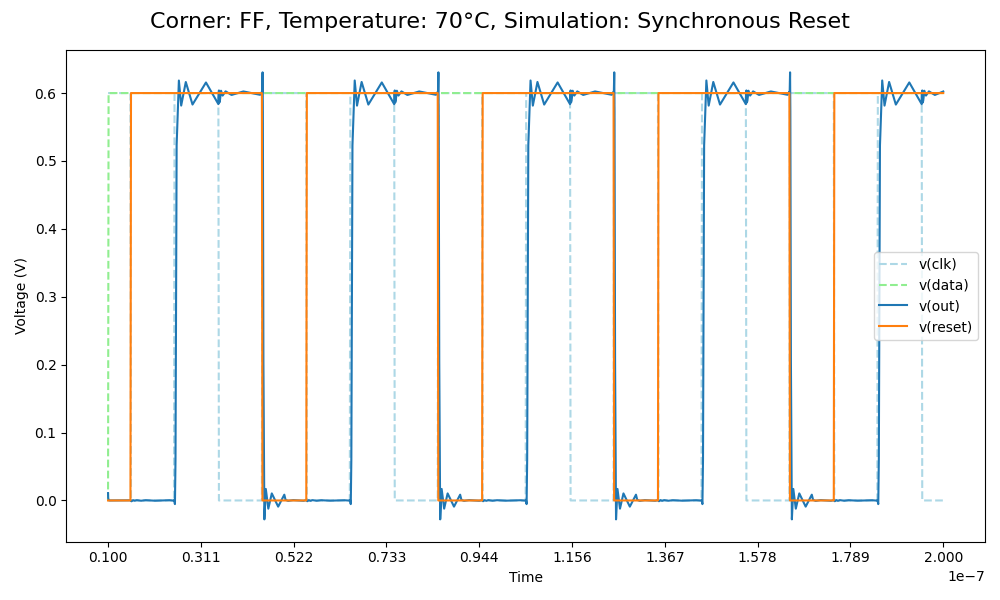
\includegraphics[height= 0.21\textheight]{figures/aimspice/0.600_0.1u_0.1u_0.3u_0.1u/functionality/FF70W3.png}
    \vspace{5pt}
    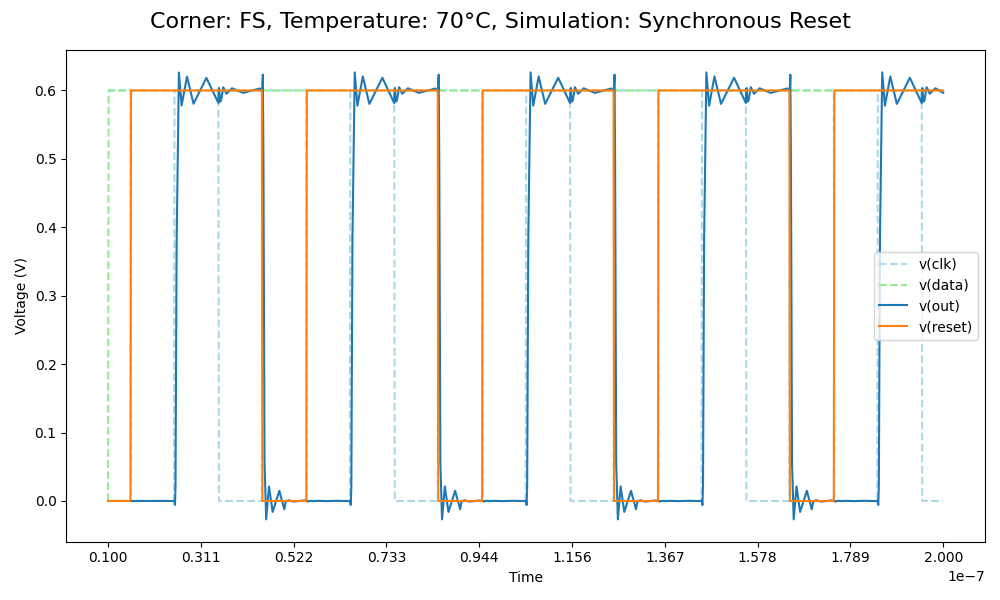
\includegraphics[height= 0.21\textheight]{figures/aimspice/0.600_0.1u_0.1u_0.3u_0.1u/functionality/FS70W3.png}
    \vspace{5pt}
    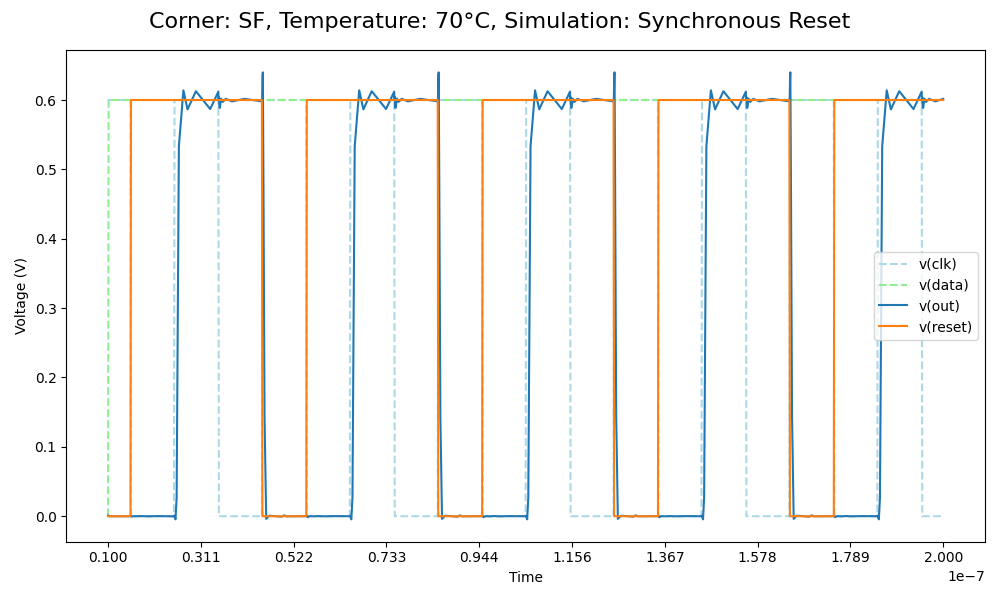
\includegraphics[height= 0.21\textheight]{figures/aimspice/0.600_0.1u_0.1u_0.3u_0.1u/functionality/SF70W3.png}
    \vspace{5pt}
    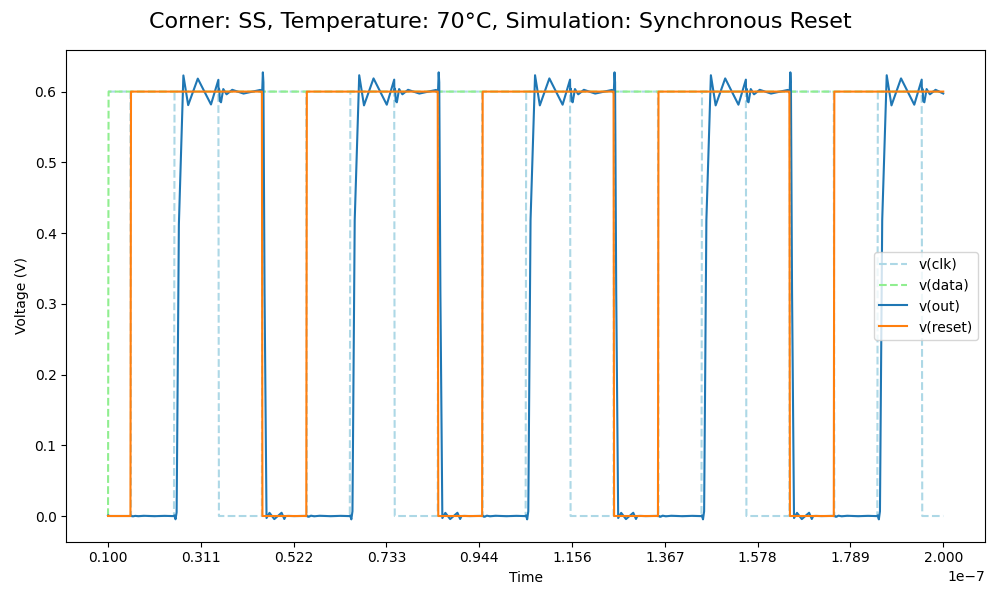
\includegraphics[height= 0.21\textheight]{figures/aimspice/0.600_0.1u_0.1u_0.3u_0.1u/functionality/SS70W3.png}
    \caption{Simulation of the reset at 70 degrees celcius.}
    \label{fig:aimspice_W3_70}
\end{figure}

